%=====================================================================
\section{Geometric reachability versus route selection}\label{sec:selection}
%=====================================================================
The results above are statements about \emph{reachability}: for each pair in a family, a route of bounded length exists, and for the families treated it is given by explicit formulas in a parameter. A different question is \emph{selection}: can a fixed rule, which sees only the current integer and a finite control state and is given no target, choose the moves so that the trajectory passes through the members of the family in order? Distance bounds and certificates are the raw material for such rules but do not by themselves provide one. We separate what is proved here from what is inherited.

\subsection{An obstruction that uses only the geometry}
\begin{theorem}[No memoryless selector]\label{thm:memoryless}
Let $\Phi:\N_{>0}\to\N_{>0}$ be any function with $\Phi(x)\in\Nbr(x)$ for all $x$. Then no orbit $x_{j+1}=\Phi(x_j)$ contains $1,2,3,\dots$ as a subsequence.
\end{theorem}
\begin{proof} Suppose the orbit contains every positive integer in order. If a value were repeated, determinism would make the orbit eventually periodic, so it would take only finitely many values, which is impossible. Hence the orbit is injective and each integer $m$ occurs at exactly one time $\tau_m$, with $\tau_1<\tau_2<\cdots$. Every term $x_j$ is a positive integer $m'$, so $j=\tau_{m'}$; if $\tau_{m+1}>\tau_m+1$, the term at a time strictly between them would be some integer $m'$ with $\tau_{m'}$ strictly between $\tau_m$ and $\tau_{m+1}$, contradicting monotonicity of $\tau$. So $\tau_{m+1}=\tau_m+1$, i.e.\ $\Phi(m)=m+1$, so $\{m,m+1\}$ is an edge. This contradicts Corollary~\ref{cor:nonadj}. \end{proof}
Only the non-adjacency of consecutive integers is used; the bound $\dist\le6$ plays no role.

\subsection{What finite control achieves (inherited)}
The same certificates provide finite-control selectors, because along every parametric route the intermediate states are strictly increasing polynomials in $t$ (in the first half of the route; one checks monotonicity symbolically), so that $t$, and hence the next label, can be recovered from the current integer and the phase. The following were established and verified in the earlier releases and are recorded here as context; they are not re-proved here.
\begin{center}\small
\begin{tabular}{@{}p{0.42\textwidth}p{0.18\textwidth}p{0.3\textwidth}@{}}\toprule
selector & control states & source\\\midrule
successor, $1,2,3,\dots$, $\le6$ moves per step & $43$ & U2-001\\
squares $1^2,2^2,\dots$, $\le5$ moves per step & $85$ & U2-SQ\\
squares via the successor selector, $\le8$ moves & $45$ & U2-SQ\\
fixed power $k$, $\le6k$ moves per step & depends on $k$ & U2-SQ\\
Fibonacci successor, from $F_k$ alone, $\le12$ moves & $99$ (path part) & U2-FP-SYM\\\bottomrule
\end{tabular}
\end{center}
The Fibonacci selector relies on a stated reading of the admissible inversion of states (a bisection on a fixed polynomial in $t$ and $A(t)=\lfloor(\sqrt{5t^2+4\varepsilon}-t)/2\rfloor$); under a stricter reading it would not apply. No selector for the primes is known. The geometry explains why the problem is different there: a selector at a prime $p$ must choose between exactly two moves, $+1$ and $+p$ (Remark~\ref{rem:primerigid}), and the distances between consecutive primes reach $8$ (Theorem~\ref{thm:primedist}).

\subsection{The distinction}
Reachability is a property of the graph; selection needs a controller with finite information about the family and arithmetic on the current state. The two are related in one direction only: the existence of certified parametric routes with recoverable parameters is what makes finite-control selection possible, but the \emph{bounds} proved in this paper do not imply it, as Theorem~\ref{thm:memoryless} shows for the simplest case.

%=====================================================================
\section{Verification and reproducibility}\label{sec:verification}
%=====================================================================
\subsection{Independent re-implementation}
Every computational statement was re-checked with new code written for this release from the definitions of Section~\ref{sec:graph} (directory \texttt{code/}); it uses neither the verifier nor the graph library of the earlier releases. The neighbour function is implemented twice (factorisation; trial division) and cross-checked against the literal definition of $E(G)$. Table~\ref{tab:checks} lists the checks and their outcomes.

\begin{table}[ht]\centering\footnotesize
\begin{tabular}{@{}p{0.07\textwidth}p{0.62\textwidth}p{0.2\textwidth}@{}}\toprule
check & content & outcome\\\midrule
C1 & neighbour function equals trial division and the literal definition of $E(G)$: $x<1500$; all pairs below $400$ ($228$ edges) & pass\\
C2 & $\deg=\tau+s$, forward and inverse neighbours distinct, no degree $3$, no loop, $\deg(1)=1$, primes have neighbours $\{4p,(p+1)^2\}$: $x<20000$ & pass\\
C3 & no triangle through any $x<10^4$; symbolic identity $a+b=(t-1)(1-ct)$; sign check; $4$-cycle and $5$-cycle; odd-cycle detection at the five vertices of the $5$-cycle & pass\\
C4 & nine identities certified symbolically (polynomial divisions, shifted non-negativity, endpoint) and replayed for $60$ values of $t$; coverage of $n\ge1$ modulo the nine classes (uncovered: $1,3$); exceptional routes; exact $\dist(n,n+1)$ for $n\le2500$ ($2\le\dist\le6$, matching the inherited table where present); $\Ball_3(163)\cap\Ball_2(164)=\emptyset$; no adjacent consecutive integers for $n<20000$ & pass\\
C5 & $24$ square identities certified symbolically and replayed for $40$ values of $t$; coverage (uncovered $1,2,3$); exceptional routes; exact $\dist(n^2,(n+1)^2)$ for $n\le150$ (matching the inherited table); $\Ball_2(529)\cap\Ball_2(576)=\emptyset$ & pass\\
C6 & scaling on $400$ random edges $\times50$ multipliers; power chains ($300$ edges, $k\le6$); $\dist(n,2n)\le5$ for $n\le30$; $\Ball_2(1)=\{1,4,16,18,25\}$ disjoint from $\Ball_2(2)$; scaling and lifting inequalities on random samples with exact distances; table $\dist(1,j)$ & pass\\
C7 & prime neighbours for $p<10^5$; reduction formula for consecutive primes below $400$; $\dist(61,67)=7$; $\dist(661,673)=8$ & pass\\
C8 & the twelve ring certificates (identities in $\Q[b][a]/(a^2+ab-b^2-\varepsilon)$ and endpoints); replay from $F_k$ for $20\le k<1500$ ($12212$ steps, all legal, ends at $F_{k+1}$, max length $12$); stored shortest paths for $2\le k\le29$; independent exact $\dist(F_k,F_{k+1})$ for $k\le25$ & pass\\
C9 & the five identities of the hand proof of Theorem~\ref{thm:famA} and their agreement with the certified class $4$ & pass\\\bottomrule
\end{tabular}
\caption{Checks run by \texttt{code/verify\_graph\_geometry.py} (about one minute). All pass; the machine-readable report is \texttt{reports/verification\_report.json}.}\label{tab:checks}\end{table}

\subsection{Status table}
\begin{table}[H]\centering\small
\begin{tabular}{@{}p{0.5\textwidth}p{0.17\textwidth}p{0.25\textwidth}@{}}\toprule
statement & status & basis\\\midrule
local finiteness, degree formula, edge ratio, non-adjacency of $n,n+1$ & proved & Section~\ref{sec:graph}; C1--C2\\
connectivity, $\dist(m,n)\le6|m-n|$ & proved from the successor bound & Theorem~\ref{thm:connected}\\
$\dist(n,n+1)\le6$ & certified & $9$ identities; C4\\
$\dist(163,164)\ge6$ & computed & ball certificate\\
scaling, product, power lifting, multiples, log bound & proved & Section~\ref{sec:mult}\\
$\dist(n,2n)\le5$ & proved & path $1\to2$, scaling\\
$\dist(1,2)\ge5$ & computed (and by hand) & balls of sizes $5$, $9$\\
$\dist(n^2,(n+1)^2)\le5$ & certified & $24$ identities; C5\\
$\dist(23^2,24^2)\ge5$ & computed & balls of sizes $97$, $562$\\
triangle-free, girth $4$, odd girth $5$ & proved & Theorems~\ref{thm:triangle}, \ref{thm:girth}\\
prime reduction & proved & Theorem~\ref{thm:primered}\\
$\dist(61,67)=7$, $\dist(661,673)=8$ & computed lower bounds, explicit paths & Theorem~\ref{thm:primedist}\\
$\dist(F_k,F_{k+1})\le12$ & certified (hand proof for one family; ring identities for the rest) & Theorem~\ref{thm:fibonacci}\\
exact small Fibonacci distances $k\le29$ & computed & Table~\ref{tab:fibsmall}\\
formal proof-assistant certification & not done & --\\\bottomrule
\end{tabular}
\caption{Status of each statement of the paper: proved (exact symbolic argument), certified (explicit identities verified exactly), computed (exact integer computation).}\label{tab:status}
\end{table}

\subsection{Inherited verifications (not re-run)}
The following earlier verifications were heavy (hours of computation) and are \emph{not} repeated here; the corresponding facts are re-checked in the ranges of Table~\ref{tab:checks} by the new code. SHA-256 of the archives, recorded in \texttt{inherited/ARCHIVE\_SHA256SUMS.txt}: U1-BND \texttt{912a068e\dots9d8e35}; U2-001 \texttt{561a9558\dots7ca21}; U2-SQ \texttt{c13a9be6\dots91733}; U2-FP-SYM \texttt{a614e196\dots2668c6}; U3-COR \texttt{038c9d11\dots4b686}. Inherited and not re-run: the successor-table verification for $n\le13500$ and the replay of the nine identities to $4\times10^5$ (U1-BND); the exact square-distance table for $n\le500$ (U2-SQ); the exact consecutive-prime and Fibonacci tables (U2-FP); the Pisano-period integrality and shifted-coefficient positivity checks of the twelve Fibonacci families (U2-FP-SYM); and the end-to-end simulations of the finite-control selectors.

\subsection{Source provenance}\label{ssec:provenance}
The earlier releases are cited at commit \texttt{22d8c2e2\dots03808} of the collection~\cite{coll}, each by its release directory. Successor distance and its sharpness: U1-BND~\cite{u1bnd}. Doubling: U2-001~\cite{u2}. Squares, scaling and power lifting: U2-SQ~\cite{u2sq}. Neighbourhoods, degrees and prime-degree rigidity: U2-TI-DYN~\cite{u2tidyn}. Prime distances and the first Fibonacci routes: U2-FP~\cite{u2fp}. The twelve certified Fibonacci families: U2-FP-SYM~\cite{u2fpsym}. Triangle-freeness and odd girth $5$: U3~\cite{u3}; the girth $4$ and the withdrawal of the value $5$: U3-COR~\cite{u3cor}, which supplements U3 and leaves it unchanged. The collection holds the release packages with their own manifests; it does not contain the present manuscript, its independent verifier, or the derived statements proved here without a release as source (the product inequality, the logarithmic bound of Corollary~\ref{cor:log}, and the cycle statement of Corollary~\ref{cor:scaledcycles}), and none of these is attributed to a release. The archive SHA-256 values of the original release archives are given in the bibliography; they are those recorded in the collection and were not recomputed here.

\subsection{Reproduction}
From the package root, \texttt{sh code/run\_all.sh} runs the verifier, regenerates the LaTeX tables from the certificate data and regenerates all figures; the manuscript is then compiled with \texttt{pdflatex} from \texttt{manuscript/}. The certificate data (identities in the form used by the verifier) are the files in \texttt{inherited/}; the verifier reads them but does not trust them: every identity is re-derived symbolically, and every route is replayed with exact integer arithmetic. Dependencies: Python $3$ with \texttt{sympy} and \texttt{matplotlib}.

%=====================================================================
\section{Mathematical significance and geometric consequences}\label{sec:significance}
%=====================================================================
\subsection{The geometry of $G$}
$G$ is a locally finite, connected, non-bipartite, triangle-free graph in which each edge multiplies the value by at least $4$. It has vertices of degree $1$, $2$ and $\ge4$ but never $3$ (Theorem~\ref{thm:degree}); multiplication by $m$ is a non-expanding self-map of $G$ (Theorem~\ref{thm:scaling}); and $x\mapsto x^k$ stretches distances by at most the factor $k$ (Theorem~\ref{thm:lifting}). Balls grow rapidly (Figure~\ref{fig:growth}: $|\Ball_4(v)|$ ranges from $119$ at $v=1$ to over $10^5$ at $v=163$), so $G$ is a sparse but very rapidly branching graph, and the geodesics between neighbouring integers climb to a large power of the endpoints and return (Figures~\ref{fig:worked} and~\ref{fig:fib}).
\begin{figure}[ht]\centering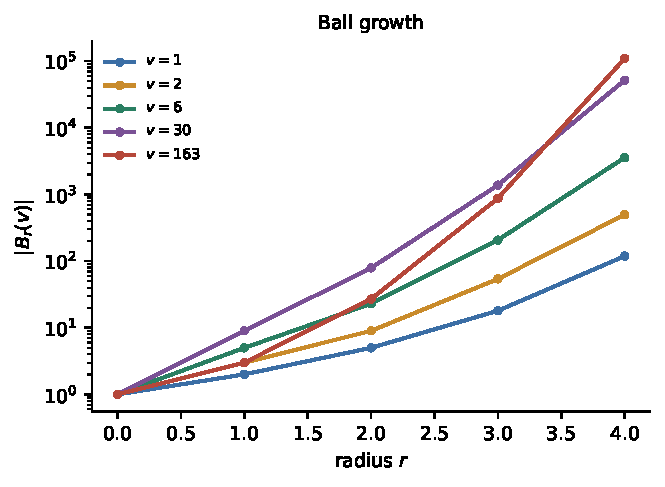
\includegraphics[width=.55\textwidth]{../figures/fig9_ball_growth.pdf}
\caption{Ball sizes $|\Ball_r(v)|$ for $r\le4$ (computed).}\label{fig:growth}\end{figure}

\subsection{Distance laws and global structure}
The three sharp laws describe one phenomenon at three scales. Integers that are adjacent as numbers are at graph distance at most $6$; an integer and its double are at distance at most $5$; and consecutive squares, although their difference grows without bound, are again at distance at most $5$. In each case the bound is exact. The successor and consecutive-square bounds follow from explicit finite families of polynomial path identities, each valid for every member of a residue class, while the doubling bound follows by multiplicative scaling of a single five-edge path. Sharpness is established by exact finite-ball certificates: the lower bound is the disjointness of two explicit balls.

These sharp local laws impose strong global metric constraints. Because $\dist(n,n+1)\le6$, the graph metric is Lipschitz in the usual absolute value, $\dist(m,n)\le6|m-n|$ (Theorem~\ref{thm:connected}); because scaling is non-expanding, the doubling and successor laws can be combined along the binary expansion of $n$, giving the logarithmic bound $\dist(1,n)\le11\lfloor\log_2n\rfloor$ (Corollary~\ref{cor:log}). Thus, although each edge multiplies by at least $4$ and by an unbounded factor $(N+1)^2/N$ in general, the diameter of $\{1,\dots,n\}$ in $(G,\dist)$ has an upper bound logarithmic in $n$. The ambient geometry of $G$ is far smaller than the Euclidean geometry of the integers, and the multiplicative structure is what makes it so: the product inequality $\dist(ab,a'b')\le\dist(a,a')+\dist(b,b')$ (Theorem~\ref{thm:product}) shows that the metric is subadditive over factorisations, and power lifting transfers a single path of length $d$ to a path of length $kd$ between $k$-th powers.

\subsection{Cycles, primes and sequences}
The shortest cycles are rigid: $G$ is triangle-free, has girth $4$, realised by $2\!-\!8\!-\!36\!-\!9$, and odd girth $5$, realised by $6\!-\!24\!-\!96\!-\!784\!-\!27$ (Theorem~\ref{thm:girth}). The impossibility of triangles is an arithmetic fact about the edge ratios: three ratios $\rho_a,\rho_b,\rho_c$ with $\rho_a\rho_b=\rho_c$ are incompatible for positive labels (Theorem~\ref{thm:triangle}).

Primes sit at the sparse end of the degree spectrum. Every prime $p$ has exactly the two neighbours $4p$ and $(p+1)^2$, so a distance between two primes is two plus a distance between composite points (Theorem~\ref{thm:primedist}); the observed values range from $4$ to $8$ for consecutive primes, with $\dist(661,673)=8$ the largest recorded, which shows that the uniform bound $6$ of the successor law is specific to consecutive integers.

Finally, the arithmetic sequences studied here are uniformly reachable: $n\to n+1$ within $6$ moves, $n\to2n$ within $5$, $n^2\to(n+1)^2$ within $5$, $n^k\to(n+1)^k$ within $6k$, and $F_k\to F_{k+1}$ within $12$ by twelve explicit formula families that are each valid for infinitely many $k$ at once. In every case the route is given by explicit integer-valued expressions in a class parameter, so reachability with a uniformly bounded number of moves is a property of the sequence itself, independent of how a route would be chosen (Section~\ref{sec:selection}).

\subsection{Relation to the multiplicative group}
If $x\sim y$ then $y/x\in\{\rho_N^{\pm1}\}$, so along any path from $x$ to $y$ the product of the edge ratios is $y/x$, and $\dist(x,y)$ is at least the word length of $y/x$ in the generators $\rho_N=(N+1)^2/N$ of the multiplicative group $\Q_{>0}$. $G$ is the part of this Cayley graph that survives the integrality requirement $N\mid x$ for forward moves, which is why the local structure depends on the divisor structure of $x$ (Theorem~\ref{thm:degree}); $G$ is not vertex-transitive, since $\deg(1)=1$, $\deg(2)=2$ and $\deg(4)=4$. Multiplication by $m$ is the natural partial symmetry: an injective graph homomorphism $G\to G$ that is not an automorphism.
The identities used throughout are certificates of a familiar kind: a rational-function parametrisation of an integral path, verified by polynomial division, whose domain of validity is a residue class.

\subsection{Proof scope and certification}
The statements of this paper are of three kinds, labelled where they occur and tabulated in Section~\ref{sec:verification}: exact symbolic proofs (the path identities, the degree formula, the scaling, lifting and cycle theorems), exact integer computations (the lower bounds $6,5,5$, the prime distances $7$ and $8$, and the tables of small cases) and inherited results (the heavy verifications of Section~\ref{sec:verification}, recorded with hashes). The lower bounds are finite computations with exact integers, cross-checked in two independent code bases; the supremum in each of the three sharp laws is attained, at $n=163$ for the successor law, at $n=1$ for doubling and at $n=23$ for squares. The Fibonacci bound $12$ is a bound on certified route length; exact distances for $k\le29$ do not exceed $6$.

\subsection{What the arithmetic graph reveals}
The operation $kN\mapsto k(N+1)^2$ looks at first like a rapidly expanding rule with no metric structure beyond growth. The results above show the opposite: the graph it generates is connected with a logarithmic upper bound on distances in integer size, is governed by three exact constants $6$, $5$, $5$ for the most natural pairs of arithmetically close integers, carries a non-expanding multiplicative action and a power-lifting inequality, has rigid shortest cycles, gives every prime exactly two neighbours, and joins consecutive Fibonacci numbers by routes of uniformly bounded length. Arithmetically close integers are geometrically close in $G$, and the proofs of this are finite, explicit and exact.

\begingroup\emergencystretch=4em\small
\begin{thebibliography}{9}
\bibitem{coll} UNNS Research Collective, \emph{UNNS Arithmetic Dynamics} (curated collection of the releases U1--U4), commit \texttt{22d8c2e23f49fb98a5b04c6b7efe9ba0a3703808}. \url{https://github.com/ukbbi/UNNS/tree/22d8c2e23f49fb98a5b04c6b7efe9ba0a3703808/projects/UNNS_ARITHMETIC_DYNAMICS}.
\bibitem{u1bnd} UNNS Research Collective, \emph{Bounded Successor Distance in the Reversible Square-Multiplication Graph}, UNNS-U1-BND, version 1.0 (v001), 8 November 2026, release \texttt{UNNS\_U1\_BND\_v001}. \url{https://github.com/ukbbi/UNNS/tree/22d8c2e23f49fb98a5b04c6b7efe9ba0a3703808/projects/UNNS_ARITHMETIC_DYNAMICS/01_metric_geometry/UNNS_U1_BND_v001}. Archive SHA-256: \path{912a068e2d26fb721c13d524f9bb18280e59a99fbafd79928781903c1c9d8e35}.
\bibitem{u2} UNNS Research Collective, \emph{Intrinsic Generative Selectors: Finite Control, Arithmetic State, and Observational Realization}, UNNS-U2-001, version 1.0 (v001), 8 November 2026, release \texttt{UNNS\_U2\_001\_v001}. \url{https://github.com/ukbbi/UNNS/tree/22d8c2e23f49fb98a5b04c6b7efe9ba0a3703808/projects/UNNS_ARITHMETIC_DYNAMICS/02_routes_selectors/UNNS_U2_001_v001}. Archive SHA-256: \path{561a9558f713faa2905be18f2a6afc2d3aac6de955c58e73cace7051e057ca21}.
\bibitem{u2sq} UNNS Research Collective, \emph{Squares and Power Sequences in the Reversible Square-Multiplication Graph}, UNNS-U2-SQ, version 1.0 (v001), 9 November 2026, release \texttt{UNNS\_U2\_SQ\_v001}. \url{https://github.com/ukbbi/UNNS/tree/22d8c2e23f49fb98a5b04c6b7efe9ba0a3703808/projects/UNNS_ARITHMETIC_DYNAMICS/02_routes_selectors/UNNS_U2_SQ_v001}. Archive SHA-256: \path{c13a9be6c9a3d1d9299a009ab08844a9840a8ec24236dd5da171806e14691733}.
\bibitem{u2tidyn} UNNS Research Collective, \emph{Maximal-Neighbor Dynamics and Prime-Degree Rigidity in the Reversible SELECT-II Arithmetic Graph}, UNNS-U2-TI-DYN, version v001, release \texttt{UNNS\_U2\_TI\_DYN\_v001}. \url{https://github.com/ukbbi/UNNS/tree/22d8c2e23f49fb98a5b04c6b7efe9ba0a3703808/projects/UNNS_ARITHMETIC_DYNAMICS/02_routes_selectors/UNNS_U2_TI_DYN_v001}. Archive SHA-256: \path{f2536563f2ed2442e969b64685a228cd68eb437bc5722d43a251ec386fe5deef}.
\bibitem{u2fp} UNNS Research Collective, \emph{Fibonacci Numbers and Primes in the Reversible Square-Multiplication Graph}, UNNS-U2-FP, version 1.0 (v001), 9 November 2026, release \texttt{UNNS\_U2\_FP\_v001}. \url{https://github.com/ukbbi/UNNS/tree/22d8c2e23f49fb98a5b04c6b7efe9ba0a3703808/projects/UNNS_ARITHMETIC_DYNAMICS/02_routes_selectors/UNNS_U2_FP_v001}. Archive SHA-256: \path{c8469e88b76c66b248c827f00edf6da07cb9af0d4daf14ed2db935951e89ee91}.
\bibitem{u2fpsym} UNNS Research Collective, \emph{Symbolic Certificates for Bounded Fibonacci Routes} (supplement to UNNS-U2-FP v001), UNNS-U2-FP-SYM, version v001, release \texttt{UNNS\_U2\_FP\_SYM\_v001}. \url{https://github.com/ukbbi/UNNS/tree/22d8c2e23f49fb98a5b04c6b7efe9ba0a3703808/projects/UNNS_ARITHMETIC_DYNAMICS/02_routes_selectors/UNNS_U2_FP_SYM_v001}. Archive SHA-256: \path{a614e196fa059bc58a7bea5bb3c616c8eaf0eead37945cb08bd56ecb982668c6}.
\bibitem{u3} UNNS Research Collective, \emph{Universal Sequence Embeddings and Structural Preservation}, UNNS-U3, version v001, release \texttt{UNNS\_U3\_v001}. \url{https://github.com/ukbbi/UNNS/tree/22d8c2e23f49fb98a5b04c6b7efe9ba0a3703808/projects/UNNS_ARITHMETIC_DYNAMICS/03_graph_structure/UNNS_U3_v001}. Archive SHA-256: \path{4f6a59b63ab58bc2842dce08289a678e63a54b22a613ea24cf0490c6ed6ee929}.
\bibitem{u3cor} UNNS Research Collective, UNNS-U3-COR (corrections to UNNS-U3 v001: girth $4$, odd girth $5$), version v001, release \texttt{UNNS\_U3\_COR\_v001}. \url{https://github.com/ukbbi/UNNS/tree/22d8c2e23f49fb98a5b04c6b7efe9ba0a3703808/projects/UNNS_ARITHMETIC_DYNAMICS/03_graph_structure/UNNS_U3_COR_v001}. Archive SHA-256: \path{038c9d1102719f3a4ee6d2afd1719ff79a9c00acb85b21b68bc98a54e454b686}.
\bibitem{wall} D.~D.~Wall, Fibonacci series modulo $m$, \emph{Amer.\ Math.\ Monthly} \textbf{67} (1960), 525--532.
\bibitem{sympy} A.~Meurer et al., SymPy: symbolic computing in Python, \emph{PeerJ Computer Science} \textbf{3}:e103 (2017).
\end{thebibliography}
\endgroup

\appendix
\section{Successor identities: states, labels and cofactors}\label{app:succ}
For each class the table lists the state before the move, the label $N$, the cofactor $c$ (so that the state before is $cN$ for $+N$ and $c(N+1)^2$ for $-N$), and the state after.
\paragraph{Class A: $n=4 t + 1$, $t\ge 1$.}
\begin{center}\small\begin{tabular}{@{}clllc@{}}\toprule
step & state before & move & cofactor $c$ & state after\\\midrule
1 & $4 t + 1$ & $+\,4 t + 1$ & $1$ & $4 \left(2 t + 1\right)^{2}$ \\
2 & $4 \left(2 t + 1\right)^{2}$ & $-\,2 t$ & $4$ & $8 t$ \\
3 & $8 t$ & $+\,t$ & $8$ & $8 \left(t + 1\right)^{2}$ \\
4 & $8 \left(t + 1\right)^{2}$ & $-\,2 t + 1$ & $2$ & $2 \left(2 t + 1\right)$ \\
\bottomrule\end{tabular}\end{center}
\paragraph{Class B: $n=8 t$, $t\ge 1$.}
\begin{center}\small\begin{tabular}{@{}clllc@{}}\toprule
step & state before & move & cofactor $c$ & state after\\\midrule
1 & $8 t$ & $+\,2$ & $4 t$ & $36 t$ \\
2 & $36 t$ & $+\,2$ & $18 t$ & $162 t$ \\
3 & $162 t$ & $-\,8$ & $2 t$ & $16 t$ \\
4 & $16 t$ & $+\,4 t$ & $4$ & $4 \left(4 t + 1\right)^{2}$ \\
5 & $4 \left(4 t + 1\right)^{2}$ & $-\,8 t + 1$ & $1$ & $8 t + 1$ \\
\bottomrule\end{tabular}\end{center}
\paragraph{Class C: $n=8 t + 2$, $t\ge 0$.}
\begin{center}\small\begin{tabular}{@{}clllc@{}}\toprule
step & state before & move & cofactor $c$ & state after\\\midrule
1 & $2 \left(4 t + 1\right)$ & $+\,2$ & $4 t + 1$ & $9 \left(4 t + 1\right)$ \\
2 & $9 \left(4 t + 1\right)$ & $+\,4 t + 1$ & $9$ & $36 \left(2 t + 1\right)^{2}$ \\
3 & $36 \left(2 t + 1\right)^{2}$ & $+\,2$ & $18 \left(2 t + 1\right)^{2}$ & $162 \left(2 t + 1\right)^{2}$ \\
4 & $162 \left(2 t + 1\right)^{2}$ & $-\,8$ & $2 \left(2 t + 1\right)^{2}$ & $16 \left(2 t + 1\right)^{2}$ \\
5 & $16 \left(2 t + 1\right)^{2}$ & $-\,8 t + 3$ & $1$ & $8 t + 3$ \\
\bottomrule\end{tabular}\end{center}
\paragraph{Class D: $n=8 t + 4$, $t\ge 0$.}
\begin{center}\small\begin{tabular}{@{}clllc@{}}\toprule
step & state before & move & cofactor $c$ & state after\\\midrule
1 & $4 \left(2 t + 1\right)$ & $+\,2$ & $2 \left(2 t + 1\right)$ & $18 \left(2 t + 1\right)$ \\
2 & $18 \left(2 t + 1\right)$ & $+\,2$ & $9 \left(2 t + 1\right)$ & $81 \left(2 t + 1\right)$ \\
3 & $81 \left(2 t + 1\right)$ & $-\,8$ & $2 t + 1$ & $8 \left(2 t + 1\right)$ \\
4 & $8 \left(2 t + 1\right)$ & $+\,2 \left(2 t + 1\right)$ & $4$ & $4 \left(4 t + 3\right)^{2}$ \\
5 & $4 \left(4 t + 3\right)^{2}$ & $-\,8 t + 5$ & $1$ & $8 t + 5$ \\
\bottomrule\end{tabular}\end{center}
\paragraph{Class E: $n=8 t + 6$, $t\ge 0$.}
\begin{center}\small\begin{tabular}{@{}clllc@{}}\toprule
step & state before & move & cofactor $c$ & state after\\\midrule
1 & $2 \left(4 t + 3\right)$ & $+\,2$ & $4 t + 3$ & $9 \left(4 t + 3\right)$ \\
2 & $9 \left(4 t + 3\right)$ & $+\,4 t + 3$ & $9$ & $144 \left(t + 1\right)^{2}$ \\
3 & $144 \left(t + 1\right)^{2}$ & $+\,2$ & $72 \left(t + 1\right)^{2}$ & $648 \left(t + 1\right)^{2}$ \\
4 & $648 \left(t + 1\right)^{2}$ & $-\,8$ & $8 \left(t + 1\right)^{2}$ & $64 \left(t + 1\right)^{2}$ \\
5 & $64 \left(t + 1\right)^{2}$ & $-\,8 t + 7$ & $1$ & $8 t + 7$ \\
\bottomrule\end{tabular}\end{center}
\paragraph{Class F: $n=24 t + 3$, $t\ge 1$.}
\begin{center}\small\begin{tabular}{@{}clllc@{}}\toprule
step & state before & move & cofactor $c$ & state after\\\midrule
1 & $3 \left(8 t + 1\right)$ & $+\,8 t + 1$ & $3$ & $12 \left(4 t + 1\right)^{2}$ \\
2 & $12 \left(4 t + 1\right)^{2}$ & $-\,4 t$ & $12$ & $48 t$ \\
3 & $48 t$ & $+\,3 t$ & $16$ & $16 \left(3 t + 1\right)^{2}$ \\
4 & $16 \left(3 t + 1\right)^{2}$ & $-\,6 t + 1$ & $4$ & $4 \left(6 t + 1\right)$ \\
\bottomrule\end{tabular}\end{center}
\paragraph{Class G: $n=8 t + 7$, $t\ge 0$.}
\begin{center}\small\begin{tabular}{@{}clllc@{}}\toprule
step & state before & move & cofactor $c$ & state after\\\midrule
1 & $8 t + 7$ & $+\,8 t + 7$ & $1$ & $64 \left(t + 1\right)^{2}$ \\
2 & $64 \left(t + 1\right)^{2}$ & $+\,t + 1$ & $64 \left(t + 1\right)$ & $64 \left(t + 1\right) \left(t + 2\right)^{2}$ \\
3 & $64 \left(t + 1\right) \left(t + 2\right)^{2}$ & $+\,t + 1$ & $64 \left(t + 2\right)^{2}$ & $64 \left(t + 2\right)^{4}$ \\
4 & $64 \left(t + 2\right)^{4}$ & $-\,2 t + 3$ & $16 \left(t + 2\right)^{2}$ & $16 \left(t + 2\right)^{2} \left(2 t + 3\right)$ \\
5 & $16 \left(t + 2\right)^{2} \left(2 t + 3\right)$ & $-\,2 t + 3$ & $4 \left(2 t + 3\right)$ & $4 \left(2 t + 3\right)^{2}$ \\
6 & $4 \left(2 t + 3\right)^{2}$ & $-\,2 \left(t + 1\right)$ & $4$ & $8 \left(t + 1\right)$ \\
\bottomrule\end{tabular}\end{center}
\paragraph{Class H: $n=24 t + 11$, $t\ge 0$.}
\begin{center}\small\begin{tabular}{@{}clllc@{}}\toprule
step & state before & move & cofactor $c$ & state after\\\midrule
1 & $24 t + 11$ & $+\,24 t + 11$ & $1$ & $144 \left(2 t + 1\right)^{2}$ \\
2 & $144 \left(2 t + 1\right)^{2}$ & $+\,24$ & $6 \left(2 t + 1\right)^{2}$ & $3750 \left(2 t + 1\right)^{2}$ \\
3 & $3750 \left(2 t + 1\right)^{2}$ & $-\,2 \left(25 t + 12\right)$ & $6$ & $12 \left(25 t + 12\right)$ \\
4 & $12 \left(25 t + 12\right)$ & $+\,25 t + 12$ & $12$ & $12 \left(25 t + 13\right)^{2}$ \\
5 & $12 \left(25 t + 13\right)^{2}$ & $-\,25 \left(2 t + 1\right)$ & $3$ & $75 \left(2 t + 1\right)$ \\
6 & $75 \left(2 t + 1\right)$ & $-\,4$ & $3 \left(2 t + 1\right)$ & $12 \left(2 t + 1\right)$ \\
\bottomrule\end{tabular}\end{center}
\paragraph{Class I: $n=24 t + 19$, $t\ge 0$.}
\begin{center}\small\begin{tabular}{@{}clllc@{}}\toprule
step & state before & move & cofactor $c$ & state after\\\midrule
1 & $24 t + 19$ & $+\,1$ & $24 t + 19$ & $4 \left(24 t + 19\right)$ \\
2 & $4 \left(24 t + 19\right)$ & $+\,24 t + 19$ & $4$ & $64 \left(6 t + 5\right)^{2}$ \\
3 & $64 \left(6 t + 5\right)^{2}$ & $-\,3$ & $4 \left(6 t + 5\right)^{2}$ & $12 \left(6 t + 5\right)^{2}$ \\
4 & $12 \left(6 t + 5\right)^{2}$ & $-\,3 \left(4 t + 3\right)$ & $3$ & $9 \left(4 t + 3\right)$ \\
5 & $9 \left(4 t + 3\right)$ & $+\,4 t + 3$ & $9$ & $144 \left(t + 1\right)^{2}$ \\
6 & $144 \left(t + 1\right)^{2}$ & $-\,6 t + 5$ & $4$ & $4 \left(6 t + 5\right)$ \\
\bottomrule\end{tabular}\end{center}


\section{Square identities: intermediate states}\label{app:sq}
For $n=24t+r$ the sequence of states $n^2=s_0,\dots,s_\ell=(n+1)^2$ along the route of Table~\ref{tab:sq}, for each $r$.
{\footnotesize\begin{description}[leftmargin=2.2em,itemsep=2pt]
\item[$r=0$] $576 t^{2} \to 48 t \left(12 t + 1\right)^{2} \to 4 \left(12 t + 1\right)^{4} \to 16 \left(12 t + 1\right)^{4} \to 4 \left(12 t + 1\right)^{2} \left(24 t + 1\right) \to \left(24 t + 1\right)^{2}$
\item[$r=1$] $\left(24 t + 1\right)^{2} \to 4 \left(288 t^{2} + 24 t + 1\right)^{2} \to 96 t \left(12 t + 1\right) \to 16 \left(6 t + 1\right)^{2} \left(12 t + 1\right) \to 4 \left(12 t + 1\right)^{2}$
\item[$r=2$] $4 \left(12 t + 1\right)^{2} \to 48 t \to 8 \left(6 t + 1\right)^{2} \to 2 \left(12 t + 1\right) \to 9 \left(8 t + 1\right)^{2}$
\item[$r=3$] $9 \left(8 t + 1\right)^{2} \to 48 \left(8 t + 1\right)^{2} \to 12 \left(8 t + 1\right)^{2} \to 96 t \to 16 \left(6 t + 1\right)^{2}$
\item[$r=4$] $16 \left(6 t + 1\right)^{2} \to 64 \left(6 t + 1\right)^{2} \to 288 \left(4 t + 1\right)^{2} \left(6 t + 1\right) \to 1296 \left(4 t + 1\right)^{4} \to 36 \left(4 t + 1\right)^{2} \left(24 t + 5\right) \to \left(24 t + 5\right)^{2}$
\item[$r=5$] $\left(24 t + 5\right)^{2} \to 4 \left(288 t^{2} + 120 t + 13\right)^{2} \to 48 \left(4 t + 1\right) \left(6 t + 1\right) \to 192 \left(3 t + 1\right)^{2} \left(4 t + 1\right) \to 36 \left(4 t + 1\right)^{2}$
\item[$r=6$] $36 \left(4 t + 1\right)^{2} \to 8 \left(6 t + 1\right) \to 32 \left(3 t + 1\right)^{2} \to 6 \left(4 t + 1\right) \to \left(24 t + 7\right)^{2}$
\item[$r=7$] $\left(24 t + 7\right)^{2} \to 4 \left(24 t + 7\right)^{2} \to 18 \left(24 t + 7\right)^{2} \to 8 \left(18 t + 5\right) \to 288 \left(3 t + 1\right)^{2} \to 64 \left(3 t + 1\right)^{2}$
\item[$r=8$] $64 \left(3 t + 1\right)^{2} \to 256 \left(3 t + 1\right)^{2} \to 1024 \left(3 t + 1\right)^{2} \to 12 \left(16 t + 5\right) \to 48 \left(8 t + 3\right)^{2} \to 9 \left(8 t + 3\right)^{2}$
\item[$r=9$] $9 \left(8 t + 3\right)^{2} \to 4 \left(288 t^{2} + 216 t + 41\right)^{2} \to 32 \left(3 t + 1\right) \left(12 t + 5\right) \to 144 \left(2 t + 1\right)^{2} \left(12 t + 5\right) \to 4 \left(12 t + 5\right)^{2}$
\item[$r=10$] $4 \left(12 t + 5\right)^{2} \to 16 \left(3 t + 1\right) \to 72 \left(2 t + 1\right)^{2} \to 2 \left(12 t + 5\right) \to \left(24 t + 11\right)^{2}$
\item[$r=11$] $\left(24 t + 11\right)^{2} \to 4 \left(24 t + 11\right)^{2} \to 18 \left(24 t + 11\right)^{2} \to 16 \left(9 t + 4\right) \to 648 \left(2 t + 1\right)^{2} \to 144 \left(2 t + 1\right)^{2}$
\item[$r=12$] $144 \left(2 t + 1\right)^{2} \to 24 \left(2 t + 1\right) \left(12 t + 7\right)^{2} \to 4 \left(12 t + 7\right)^{4} \to 16 \left(12 t + 7\right)^{4} \to 4 \left(12 t + 7\right)^{2} \left(24 t + 13\right) \to \left(24 t + 13\right)^{2}$
\item[$r=13$] $\left(24 t + 13\right)^{2} \to 4 \left(288 t^{2} + 312 t + 85\right)^{2} \to 48 \left(2 t + 1\right) \left(12 t + 7\right) \to 64 \left(3 t + 2\right)^{2} \left(12 t + 7\right) \to 4 \left(12 t + 7\right)^{2}$
\item[$r=14$] $4 \left(12 t + 7\right)^{2} \to 24 \left(2 t + 1\right) \to 32 \left(3 t + 2\right)^{2} \to 2 \left(12 t + 7\right) \to 9 \left(8 t + 5\right)^{2}$
\item[$r=15$] $9 \left(8 t + 5\right)^{2} \to 48 \left(8 t + 5\right)^{2} \to 12 \left(8 t + 5\right)^{2} \to 48 \left(2 t + 1\right) \to 64 \left(3 t + 2\right)^{2}$
\item[$r=16$] $64 \left(3 t + 2\right)^{2} \to 256 \left(3 t + 2\right)^{2} \to 576 \left(3 t + 2\right) \left(4 t + 3\right)^{2} \to 1296 \left(4 t + 3\right)^{4} \to 36 \left(4 t + 3\right)^{2} \left(24 t + 17\right) \to \left(24 t + 17\right)^{2}$
\item[$r=17$] $\left(24 t + 17\right)^{2} \to 4 \left(288 t^{2} + 408 t + 145\right)^{2} \to 96 \left(3 t + 2\right) \left(4 t + 3\right) \to 48 \left(4 t + 3\right) \left(6 t + 5\right)^{2} \to 36 \left(4 t + 3\right)^{2}$
\item[$r=18$] $36 \left(4 t + 3\right)^{2} \to 16 \left(3 t + 2\right) \to 8 \left(6 t + 5\right)^{2} \to 6 \left(4 t + 3\right) \to \left(24 t + 19\right)^{2}$
\item[$r=19$] $\left(24 t + 19\right)^{2} \to 4 \left(24 t + 19\right)^{2} \to 18 \left(24 t + 19\right)^{2} \to 16 \left(9 t + 7\right) \to 72 \left(6 t + 5\right)^{2} \to 16 \left(6 t + 5\right)^{2}$
\item[$r=20$] $16 \left(6 t + 5\right)^{2} \to 32 \left(3 t + 2\right) \to 288 \left(t + 1\right)^{2} \to 18 \left(4 t + 3\right) \to 9 \left(8 t + 7\right)^{2}$
\item[$r=21$] $9 \left(8 t + 7\right)^{2} \to 4 \left(288 t^{2} + 504 t + 221\right)^{2} \to 16 \left(6 t + 5\right) \left(12 t + 11\right) \to 576 \left(t + 1\right)^{2} \left(12 t + 11\right) \to 4 \left(12 t + 11\right)^{2}$
\item[$r=22$] $4 \left(12 t + 11\right)^{2} \to 8 \left(6 t + 5\right) \to 288 \left(t + 1\right)^{2} \to 2 \left(12 t + 11\right) \to \left(24 t + 23\right)^{2}$
\item[$r=23$] $\left(24 t + 23\right)^{2} \to 4 \left(24 t + 23\right)^{2} \to 18 \left(24 t + 23\right)^{2} \to 8 \left(18 t + 17\right) \to 2592 \left(t + 1\right)^{2} \to 576 \left(t + 1\right)^{2}$
\end{description}}


\section{Fibonacci data}\label{app:fib}
The labels of the twelve certified families are in Section~\ref{ssec:fibfamilies}; the states $s_i\in O_\varepsilon$ in normal form $p_0(b)+p_1(b)a$ are in \texttt{inherited/u2fpsym\_class\_certificates.json} (key \texttt{states\_ring}). The exact distances for $k\le29$ are in Table~\ref{tab:fibsmall}.

\section{Package contents}
\begin{description}[leftmargin=1.6em,itemsep=1pt]
\item[\texttt{manuscript/}] LaTeX source and compiled PDF.
\item[\texttt{figures/}] all figures (PDF, PNG) and the script \texttt{code/make\_figures.py}.
\item[\texttt{tables/}] generated LaTeX tables (\texttt{code/make\_tables.py}).
\item[\texttt{code/}] \texttt{ugraph.py} (graph engine), \texttt{verify\_graph\_geometry.py}, \texttt{run\_all.sh}.
\item[\texttt{data/}] independently computed distance tables.
\item[\texttt{inherited/}] unchanged copies of the certificate data and earlier code, with a hash list.
\item[\texttt{reports/}] verification report and verifier output.
\end{description}
\end{document}
